\documentclass[tikz,border=5]{standalone}

\begin{document}

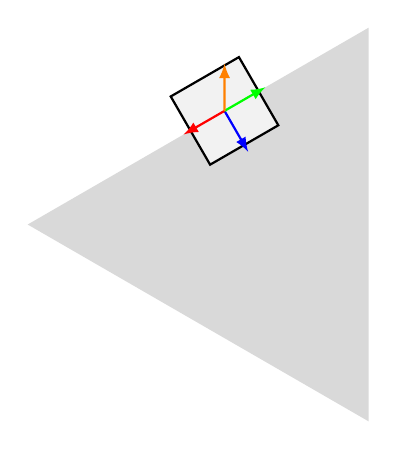
\begin{tikzpicture}
    % Parameters
    \def\angle{30} % angle of incline
    \def\boxSize{1} % size of the box
    \def\forceScale{0.6} % scale for the force vectors

    % Define the ramp
    \fill[gray!30] (0,0) --++ (\angle:5) --++ (0,-5) -- cycle;

    % Place the box at the middle of the ramp
    \begin{scope}[shift={(2.5,2.5*tan(\angle))},rotate=\angle]
        \draw[thick,fill=gray!10] (-\boxSize/2,-\boxSize/2) rectangle ++(\boxSize,\boxSize);
        % Forces
        \draw[thick,blue,-latex] (0,0) --++ (0,-\forceScale); % weight
        \draw[red,thick,-latex] (0,0) --++ (-\forceScale,0); % friction
        \draw[green,thick,-latex] (0,0) --++ (\forceScale,0); % applied force
        \draw[orange,thick,-latex](0,0) --++ (90-\angle:\forceScale); % normal force
    \end{scope}
\end{tikzpicture}

\end{document}